%!TEX root = ../../da.tex

\chapter{Heat Flux}
\label{ch:gk-hf}

% {\normalfont[...]}
\begin{chapquote}{M.P. Allen, \textit{Computer Simulations in Chemical Physics}}
	 \el there are many subtleties associated with the calculation of transport coefficients in computer simulations. These subtleties cannot be completely divorced from a consideration of the boundary conditions.
\end{chapquote}

\begin{chapquote}{Sonic the Hedgehog, \textit{Sonic X Theme Song}}
	\noindent
	Gotta Go Fast!
\end{chapquote}

\noindent
As we have seen in \cref{ch:gk}, the instantaneous heat flux $\J(t)$ is the central quantity required to compute thermal conductivities with the \gls{gk} method.
Its formulation and implementation for different types of potential has been the focus of much previous work.

\newthought{Initial efforts by Irving and Kirkwood}~\cite{ik1950t}, later formalised by Noll~\cite{n1955t}, and continued by others~\cite{h1982t,mb1993p,at2010p,fs2015t} were undertaken within the wider context of establishing a connection between continuum descriptions and statistical mechanics.
These early works assumed additive pairwise potentials, leading to first \gk simulations with such potentials~\cite{agw1970t,lvk1973t,lmh1986t}.
Shortly after, Hardy established a form of the heat flux for periodic quantum systems~\cite{h1963t} without this assumption.
However, this form was not straightforward to apply to the non-pairwise many-body \ffs (see \cref{sec:ffs}) developed in the late 1980s~\cite{sw1985p,t1988p,b1990p}.
This lead to the development of many differing forms of the heat flux for such cases, often based on extensions of stress-based formulas developed for pairwise potentials~\cite{vc1999t,c2006t,ggs2010t,fpdh2015t}.

It has only recently been widely acknowledged that such many-body potentials, or, more precisely, those which are not composed of additive pairwise terms, require a fundamentally different treatment.
Fan~\etal~\cite{fpdh2015t} showed that the classical equivalent of the formulation by Hardy~\cite{h1963t} provides a general heat flux, unifying previous formulations for many-body potentials, and highlighting the distinction between stress-based pairwise and general Hardy-like formulas.
Boone \etal~\cite{bbw2019t} investigated previous heat flux formulations in the \gls{lammps} code, finding that a heat flux for pairwise potentials is incorrect for many-body potentials. Based on a derivation by Toori~\etal~\cite{tno2008t}, they provide a heat flux for three- and four-body potentials.
Surblys \etal~\cite{smko2019t} provide an alternative \scare{centroid} formulation for \gls{lammps}, also based on the work by Toori \etal~\cite{tno2008t}.

In parallel, heat flux formulations for \dft were developed, enabling \gls{aigk} calculations~\cite{mub2016t,crs2017t}.
% The recent observation that the gauge freedom of the energy density~\cite{cm1992t} leads to terms in the heat flux that do not contribute to $\tk$ can be used to discard irrelevant, seemingly different terms~\cite{mub2016t,emub2016t}.

\newthought{This complex landscape} of different forms of the heat flux, and different perspectives on its derivation, presents a challenge for the present work. 
Here, we seek to develop a heat flux for \mlps in general and \glps in particular, under the constraint that derivatives are computed with \ad, rather than manually implemented.
While some existing forms can be applied in principle to this case, doing so is not straightforward and can lead to high computational cost, as we will highlight over the course of this section.\marginnote{A discussion of selected heat flux formulations and their relationship to the ones discussed in this work is given in \cref{sec:si-heat_flux_literature}.} Nomenclature differs significantly across existing forms, and periodicity is often treated only implicitly, leading to potential ambiguities in implementation.

\newthought{In this section,} we aim to clarify the formulation of the heat flux for classical many-body potentials, including semi-local \glps, and provide guidelines for the efficient and simple implementation of the result with \ad. An instructive implementation in \texttt{jax}~\cite{jax} is provided in the \texttt{glp} package (see \cref{sec:si-glp}).

To this end, we proceed in two stages:
In the first part of this section, \cref{sec:hf_outline,sec:hf_dense,sec:hf_ceqn,sec:hf_integrate,sec:hf_terms}, the Hardy heat flux formulation is re-derived with a particular emphasis on an explicit treatment of periodicity and consistent nomenclature.
In the second part, \cref{sec:hf_imp,sec:hf_mic,sec:hf_glps,sec:hf_unf}, strategies for the efficient implementation of the result are discussed, and a linear-scaling formulation using \ad for local and semi-local \glps is developed.
\Cref{sec:hf_summary} provides a summary of results.

\section{Setting the Problem}
\label{sec:hf_outline}

The heat flux required for the \gls{gk} method was introduced in \cref{ch:gk} as the spatial integral of a heat current density $\densj(\R, t)$, which arises from a continuity equation, \cref{eq:gk-ceqn}, for the energy density $\dense(\R, t)$, which in turn is defined as a scalar field that integrates to the total energy of the system $E$.
Obtaining the heat flux therefore requires \emph{(a)} making an ansatz for $\dense(\R, t)$, \emph{(b)} solving the continuity equation for $\densj(\R,t)$, and \emph{(c)} executing the spatial integral to obtain $\J(t)$.


% The heat flux required for the \gls{gk} method was introduced in the previous chapter as the spatial integral of a heat current density
% \begin{equation}
% 	\J(t) = \integral{V}^3r \, \densj(\R, t) \, ,
% \end{equation}
% which arises from a continuity equation for the energy density
% \begin{equation}
% 	\dot e(\R, t) + \boldsymbol{\nabla} \cdot \boldsymbol{j}(\R, t) = 0 \, , \label{eq:hf-ceqn}
% \end{equation}
% which in turn is defined as a scalar field that integrates to the total energy of the system
% \begin{equation}
% 	E(t) = \integral{V}^3r \, e(\R, t) \, .
% \end{equation}

Overall, these steps follow a later approach by Hardy~\cite{h1982t}, which the present works extends to non-pairwise potentials. Explicitly separating the computation of the heat current density from the integration allows us to introduce periodicity in a controlled manner, using the notation established in \cref{ch:pbc}.

\clearpage
\section{Defining the Energy Density}
\label{sec:hf_dense}

\marginnote{We now adopt the notation of \cref{ch:md}, treating a system with $N$ atoms contained in a volume $V$; the bulk limit will be considered later. Recall that the energy depends on time through atomic positions (potential energy) and the velocities (kinetic energy); there is no explicit time dependence in this setting. We therefore drop explicit mentions of $t$, for instance writing $\dense(\R)$ instead of $\dense(\R, t)$.}
Conceptually, defining $\dense(\R)$ requires a formal connection between a continuum (or \emph{hydrodynamical}) description in terms of spatially continuous densities, and the statistical mechanics (or \md) description in terms of statistical ensembles of point particles.
% This task extends well beyond the \gk method.
While details vary across methods,\footnote{An early introduction to such approaches is given by Noll~\cite{n1955t}. A recent overview can be found in reference~\cite{fs2015t}.} the essential idea is to use \newterm{localisation functions} $\localf{\R_i - \R}$, which are peaked at $\R_i$, decay to $0$ as $|\R - \R_i|$ increases, and are normalised to $1$, to formally map quantities assigned to discrete atoms $i$ to densities.

In the case of inhomogeneous systems with atomically sharp interfaces or non-equilibrium approaches, the microscopic\footnote{On the scale of single atoms, as opposed to the simulation cell.} details of localisation function and averaging approach gain central importance~\cite{cd2016t}. The \gk method, however, is concerned with system-wide averages and equilibrium \md, and we therefore use generic localisation functions, not relying on any particular form.

 % we can therefore adopt a simplified approach by Hardy~\cite{h1982t}.

The usage of localisation functions requires the ability to assign contributions to the total energy $E$ to atomic positions,\footnote[][-2\baselineskip]{We note in passing that one does not necessarily need to rely on atomic positions. Recent work by Surblys~\etal{}~\cite{smko2019t}, for instance, assigns potential energy contributions arising from groups of atoms to their centre of mass. In \cref{sec:hf_terms}, we will also see that in solids, it is useful to assign atomic potential energies to fixed, rather than instantaneous, positions. Nevertheless, access to some form of contributions to $U$ is required.} which is straightforward for the kinetic energy\footnote{Recall that in the framework of \md as described in \cref{ch:md}, nuclei are treated as classical point particles with kinetic energy $T_i = 1/2\, m_i \V_i^2$.} $T$, but not for the potential energy $U$.

To proceed, we restrict the present derivation to potentials constructed \emph{a priori} from atomic contributions
\begin{equation}
	U(\Rgen) = \sum_{i=1}^N U_i(\Rgen) \, . \label{eq:hf_u_gen}
\end{equation}
For now, these contributions can be an arbitrary many-body function of all $N$ atomic positions $\Rgen$.
This setting differs from the case of \dft, where an energy density can be defined~\cite{cm1992t}, but no direct decomposition of the total energy into atomic contributions is available.\footnote[][]{The derivation of the heat flux therefore proceeds differently. Carborgno~\etal~\cite{crs2017t} exploit the structure of the Hamiltonian in \cref{eq:qm-he}, which consists of one- and two-body terms involving atomic and electronic degrees of freedom, to define atomic contributions to the Hellmann-Feynman forces and thereby obtain a heat flux for solids. Marcolongo~\etal~\cite{mub2016t} proceed from the energy density directly, obtaining a numerically more involved heat flux.}
Previous discussions of the heat flux have been concerned with the question of uniqueness arising from the arbitrary partitioning of a given total potential energy into atomic contributions.
For potentials explicitly composed of two- or three-body contributions, numerical experiments~\cite{h2012t} and the gauge principle~\cite{emub2016t} have shown that the exact composition of atomic contributions has no impact on the thermal conductivity.
In the case of \mlps, $U_i$ may be many-body functions without any further decomposition into $k$-body contributions.
Therefore, a given partitioning into $U_i$ must be considered as-is.\footnote{Re-partitioning can in principle be performed by defining an additional function that redistributes energy between atoms, which may be advantageous for the purpose of \gk convergence~\cite{meb2020t}. In that case, the thermal conductivity remains unchanged if such a change corresponds to a non-diffusive flux as discussed in \cref{sec:gk-gauge}. At present, this is not pursued.}

With these considerations, we are now in a position to make the ansatz for the energy density
\begin{equation}
	\dense(\R) = \sum_{i=1}^N \localf{\R_i - \R} \left(U_i + T_i\right) = \sum_{i=1}^N \localf{\R_i - \R} E_i \, .
\end{equation}


\section{Solving the Continuity Equation}
\label{sec:hf_ceqn}

The next step is solving \cref{eq:gk-ceqn}, which we accomplish by re-writing the time derivative of $\dense(\R)$ in a form that can be directly identified as the divergence of the heat current density $\densj(\R)$, and therefore the solution of the continuity equation.

\noindent
To this end, we first define a \newterm{bond function}:\footnote{In essence, a bond function gives a contribution only where $\R$ lies on the line segment between $\R_i$ and $\R_j$. It can be seen as the two-dimensional equivalent of the localisation function.}
\begin{equation}
	\bondf{ij}{\R} = \int_0^1 \, \text{d} \lambda\, \localf{\lambda \R_i + (1-\lambda) \R_j - \R} \, .
\end{equation}
One can then show that\footnote[][2\baselineskip]{A more rigorous derivation of similar relations is given by Noll in~\cite{n1955t}, based on the work of Irving and Kirkwood~\cite{ik1950t}. A short proof is provided in \cref{sec:si-hf_identities}.}
\begin{equation}
	\localf{\R_i - \R} - \localf{\R_j - \R} = \R_{ij} \cdot \grad_{\R} \bondf{ij}{\R} \, . \label{eq:hf_bondf_identity}
\end{equation}
With this identity, any term that can be written in terms of a difference at two locations $\R_i$ and $\R_j$ can be identified as a heat flux along the line segment between them.

The time-derivative of $\dense(\R)$ is
\begin{equation}
	\totaldiff{t} \dense(\R, t) = \sum_{i=1}^N \left(\totaldiff{t} E_i\right) \localf{\R_i - \R} + \sum_{i=1}^N E_i \left(\totaldiff{t} \localf{\R_i - \R} \right) \, .
\end{equation}
The first term can be tackled by splitting $E_i = U_i + T_i$ and resolving the time derivative (see \cref{sec:si-hf_dt_dense})\marginnote{Note that this manipulation relies on the ability to freely rename $i$ and $j$, as both appear in a sum running over $1...N$. For this reason, we have not yet transitioned to a periodic system.}
\begin{align}
	&\sum_{i=1}^N \left(\totaldiff{t} E_i\right) \localf{\R_i - \R}  \\
	&= \sum_{i,j=1}^N \left[\left(\dur{i}{j}{} \cdot \V_j\right)  \left(\localf{\R_i - \R} - \localf{\R_j - \R}\right) \right] \, ,
\end{align}
and finally applying the identity from \cref{eq:hf_bondf_identity} to obtain
\begin{equation}
	= \grad_{\R} \cdot \left[\sum_{i,j=1}^N \R_{ij} \left(\dur{i}{j}{} \cdot \V_j\right) \bondf{ij}{\R} \right] \, .
\end{equation}
The second term is resolved by the chain rule
\begin{align}
	\sum_{i=1}^N E_i \left(\totaldiff{t} \localf{\R_i - \R} \right) &= -\sum_{i=1}^N E_i \Big( \grad_{\R} \localf{\R_i - \R} \cdot \V_i \Big) \\
	&= -\grad_{\R} \cdot \Big( \sum_{i=1}^N E_i \localf{\R_i - \R} \V_i \Big) \, .
\end{align}
Comparing with \cref{eq:gk-ceqn}, we find\marginnote{Note the flipped signs.}
\begin{equation}
	\densj(\R) = \sum_{i,j=1}^N \R_{ji} \left(\dur{i}{j}{} \cdot \V_j\right) \bondf{ij}{\R} + \sum_{i=1}^N E_i \V_i \localf{\R_i - \R} \, . \label{eq:hf_densj}
\end{equation}

\newthought{While so far we} have relied on purely algebraic manipulations, this result can also be justified from a physical perspective. Any energy change at atom $i$ must be balanced out by corresponding changes in the atoms $j$ it interacts with, with an energy current flowing between them.\footnote[][-3\baselineskip]{This does not mean that pairwise fluxes are always zero -- this is only the case if $\indur{i}{j}{} = \indur{j}{i}{}$, which only applies to pair potentials. In general, the energy change in $i$ is divided up in some way between its neighbours.} If we can divide up the change in $U_i$ into contributions that can be attributed to different $j$, and identify the corresponding terms in $U_j$, we know the magnitude of the current between $i$ and $j$. It is a natural assumption that the current flows directly between them, parallel to $\R_{ij}$.
The first term in \cref{eq:hf_densj} is one way to construct a vector field accordingly.
The second term describes an alternative process to change local distribution of energy: Rather than energy flowing between atoms, the energy situated at a given atom is \scare{dragged along} by the atom moving. Together, these two processes describe how the energy density can change, and therefore yield the heat current density, solving the continuity equation.

\section{Heat Flux in the Bulk}
\label{sec:hf_integrate}

At this point, $\densj(\R)$ has been obtained for $N$ particles with open boundary conditions.
As discussed in \cref{ch:pbc}, practical simulations of bulk systems, however, are performed in a periodic setting.
We therefore adopt the notation established in that section, obtaining
\begin{equation}
	\densj^{\text{bulk}}(\R) = \sum_{\substack{i \in \Rall \\ j \in \Rall}} \R_{ji} \left(\dur{i}{j}{} \cdot \V_j\right) \bondf{ij}{\R} + \sum_{i \in \Rall} E_i \V_i \localf{\R_i - \R} \, . \label{eq:hf_densj_bulk}
\end{equation}
The result is illustrated in \cref{fig:hf_densj}.
\begin{figure}
  \centering
  
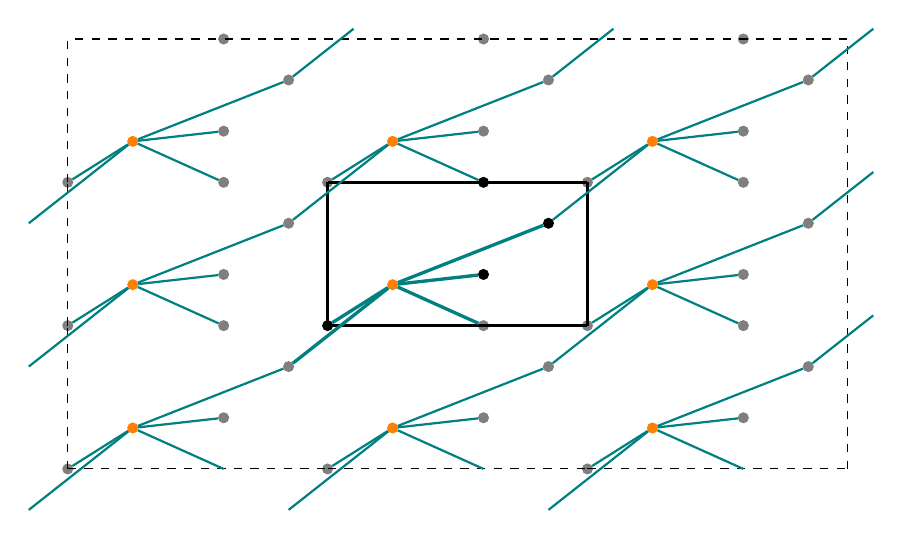
\begin{tikzpicture}[
    x = 1.65cm,
    y = 1.3cm,
    >=stealth,
    atom/.style = {circle, fill=black, minimum size=4pt,
    inner sep=0pt, outer sep=0pt},
    replica/.style = {circle, fill=black, minimum size=4pt,
    inner sep=0pt, outer sep=0pt, opacity=0.5},
]

\node[replica] (rep_0_00) at (0.0,0.0){};
    \node[replica, fill=orange, opacity=1] (rep_1_00) at (0.5,0.4){};
    \node[replica] (rep_2_00) at (1.2,0.5){};
    \node[replica] (rep_3_00) at (1.2,1.4){};
    \node[replica] (rep_4_00) at (1.7,1.0){};
    \draw [dashed] (0.0,0.0) -- (2.0,0.0);
    \draw [dashed] (0.0,0.0) -- (0.0,1.4);
    \node[replica] (rep_0_01) at (0.0,1.4){};
    \node[replica, fill=orange, opacity=1] (rep_1_01) at (0.5,1.7999999999999998){};
    \node[replica] (rep_2_01) at (1.2,1.9){};
    \node[replica] (rep_3_01) at (1.2,2.8){};
    \node[replica] (rep_4_01) at (1.7,2.4){};
    % \draw [dashed] (0.0,1.4) -- (2.0,1.4);
    \draw [dashed] (0.0,1.4) -- (0.0,2.8);
    \node[replica] (rep_0_02) at (0.0,2.8){};
    \node[replica, fill=orange, opacity=1] (rep_1_02) at (0.5,3.1999999999999997){};
    \node[replica] (rep_2_02) at (1.2,3.3){};
    \node[replica] (rep_3_02) at (1.2,4.199999999999999){};
    \node[replica] (rep_4_02) at (1.7,3.8){};
    % \draw [dashed] (0.0,2.8) -- (2.0,2.8);
    \draw [dashed] (0.0,2.8) -- (0.0,4.199999999999999);
    \node[replica] (rep_0_10) at (2.0,0.0){};
    \node[replica, fill=orange, opacity=1] (rep_1_10) at (2.5,0.4){};
    \node[replica] (rep_2_10) at (3.2,0.5){};
    \node[replica] (rep_3_10) at (3.2,1.4){};
    \node[replica] (rep_4_10) at (3.7,1.0){};
    \draw [dashed] (2.0,0.0) -- (4.0,0.0);
    % \draw [dashed] (2.0,0.0) -- (2.0,1.4);
    \node[atom] (atom_0) at (2.0,1.4){};
    \node[atom, fill=orange, opacity=1] (atom_1) at (2.5,1.7999999999999998){};
    \node[atom] (atom_2) at (3.2,1.9){};
    \node[atom] (atom_3) at (3.2,2.8){};
    \node[atom] (atom_4) at (3.7,2.4){};
    % \draw [dashed] (2.0,1.4) -- (4.0,1.4);
    % \draw [dashed] (2.0,1.4) -- (2.0,2.8);
    \node[replica] (rep_0_12) at (2.0,2.8){};
    \node[replica, fill=orange, opacity=1] (rep_1_12) at (2.5,3.1999999999999997){};
    \node[replica] (rep_2_12) at (3.2,3.3){};
    \node[replica] (rep_3_12) at (3.2,4.199999999999999){};
    \node[replica] (rep_4_12) at (3.7,3.8){};
    % \draw [dashed] (2.0,2.8) -- (4.0,2.8);
    % \draw [dashed] (2.0,2.8) -- (2.0,4.199999999999999);
    \node[replica] (rep_0_20) at (4.0,0.0){};
    \node[replica, fill=orange, opacity=1] (rep_1_20) at (4.5,0.4){};
    \node[replica] (rep_2_20) at (5.2,0.5){};
    \node[replica] (rep_3_20) at (5.2,1.4){};
    \node[replica] (rep_4_20) at (5.7,1.0){};
    \draw [dashed] (4.0,0.0) -- (6.0,0.0);
    % \draw [dashed] (4.0,0.0) -- (4.0,1.4);
    \node[replica] (rep_0_21) at (4.0,1.4){};
    \node[replica, fill=orange, opacity=1] (rep_1_21) at (4.5,1.7999999999999998){};
    \node[replica] (rep_2_21) at (5.2,1.9){};
    \node[replica] (rep_3_21) at (5.2,2.8){};
    \node[replica] (rep_4_21) at (5.7,2.4){};
    % \draw [dashed] (4.0,1.4) -- (6.0,1.4);
    % \draw [dashed] (4.0,1.4) -- (4.0,2.8);
    \node[replica] (rep_0_22) at (4.0,2.8){};
    \node[replica, fill=orange, opacity=1] (rep_1_22) at (4.5,3.1999999999999997){};
    \node[replica] (rep_2_22) at (5.2,3.3){};
    \node[replica] (rep_3_22) at (5.2,4.199999999999999){};
    \node[replica] (rep_4_22) at (5.7,3.8){};
    % \draw [dashed] (4.0,2.8) -- (6.0,2.8);
    % \draw [dashed] (4.0,2.8) -- (4.0,4.199999999999999);
    \draw [solid, very thick] (2.0,1.4) -- (4.0,1.4);
\draw [solid, very thick] (4.0,1.4) -- (4.0,2.8);
\draw [solid, very thick] (4.0,2.8) -- (2.0,2.8);
\draw [solid, very thick] (2.0,2.8) -- (2.0,1.4);
\draw [dashed] (6.0,0.0) -- (6.0,4.199999999999999);
\draw [dashed] (6.0,4.199999999999999) -- (0.0,4.199999999999999);

\draw [teal, solid, very thick] (atom_1) -- (atom_0);
\draw [teal, solid, very thick] (atom_1) -- (atom_2);
\draw [teal, solid, very thick] (atom_1) -- (atom_4);
\draw [teal, solid, very thick] (atom_1) -- (rep_3_10);
\draw [teal, solid, very thick] (atom_1) -- (rep_4_00);

% 2.5, 1.8 - 3.2, 1.4 = +0.7, -0.4
% 2.5, 1.8 - 1.7, 1.0 = +0.8, +0.8

\draw [teal, solid, thick] (rep_1_22) -- (rep_0_22);
\draw [teal, solid, thick] (rep_1_22) -- (rep_2_22);
\draw [teal, solid, thick] (rep_1_22) -- (rep_4_22);
\draw [teal, solid, thick] (rep_1_22) -- (atom_4);
\draw [teal, solid, thick] (rep_1_22) -- (rep_3_21);

\draw [teal, solid, thick] (rep_1_21) -- (rep_0_21);
\draw [teal, solid, thick] (rep_1_21) -- (rep_2_21);
\draw [teal, solid, thick] (rep_1_21) -- (rep_4_21);
\draw [teal, solid, thick] (rep_1_21) -- (rep_4_10);
\draw [teal, solid, thick] (rep_1_21) -- (rep_3_20);

\draw [teal, solid, thick] (rep_1_20) -- (rep_0_20);
\draw [teal, solid, thick] (rep_1_20) -- (rep_2_20);
\draw [teal, solid, thick] (rep_1_20) -- (rep_4_20);
\draw [teal, solid, thick] (rep_1_20) -- (3.7,-0.4);
\draw [teal, solid, thick] (rep_1_20) -- (5.2,0.0);


\draw [teal, solid, thick] (rep_1_10) -- (rep_0_10);
\draw [teal, solid, thick] (rep_1_10) -- (rep_2_10);
\draw [teal, solid, thick] (rep_1_10) -- (rep_4_10);
\draw [teal, solid, thick] (rep_1_10) -- (1.7,-0.4);
\draw [teal, solid, thick] (rep_1_10) -- (3.2,0.0);

\draw [teal, solid, thick] (rep_1_00) -- (rep_0_00);
\draw [teal, solid, thick] (rep_1_00) -- (rep_2_00);
\draw [teal, solid, thick] (rep_1_00) -- (rep_4_00);
\draw [teal, solid, thick] (rep_1_00) -- (-0.3,-0.4);
\draw [teal, solid, thick] (rep_1_00) -- (1.2,0.0);


\draw [teal, solid, thick] (rep_1_01) -- (rep_0_01);
\draw [teal, solid, thick] (rep_1_01) -- (rep_2_01);
\draw [teal, solid, thick] (rep_1_01) -- (rep_4_01);
\draw [teal, solid, thick] (rep_1_01) -- (-0.3,1.0);
\draw [teal, solid, thick] (rep_1_01) -- (rep_3_00);

\draw [teal, solid, thick] (rep_1_02) -- (rep_0_02);
\draw [teal, solid, thick] (rep_1_02) -- (rep_2_02);
\draw [teal, solid, thick] (rep_1_02) -- (rep_4_02);
\draw [teal, solid, thick] (rep_1_02) -- (-0.3,2.4);
\draw [teal, solid, thick] (rep_1_02) -- (rep_3_01);


\draw [teal, solid, thick] (rep_1_12) -- (rep_0_12);
\draw [teal, solid, thick] (rep_1_12) -- (rep_2_12);
\draw [teal, solid, thick] (rep_1_12) -- (rep_4_12);
\draw [teal, solid, thick] (rep_1_12) -- (rep_4_01);
\draw [teal, solid, thick] (rep_1_12) -- (atom_3);

% bonus: draw lines extending out up to some arbitrary tolerance

\draw [teal, solid, thick] (rep_4_20) -- (6.2,1.5);
\draw [teal, solid, thick] (rep_4_21) -- (6.2,2.9);
\draw [teal, solid, thick] (rep_4_22) -- (6.2,4.3);
\draw [teal, solid, thick] (rep_4_12) -- (4.2,4.3);
\draw [teal, solid, thick] (rep_4_02) -- (2.2,4.3);


\end{tikzpicture}

  \caption{
  Illustration of the first term of the bulk current density in \cref{eq:hf_densj_bulk}, showing bond functions as lines connecting atoms.
  The system from \cref{fig:glp-mpnn_sketch} is used, assuming that $U_i$ depends on interactions up to $\interactions{=}2$. Only bond functions involving the atom highlighted in orange and its replicas are shown. The simulation cell and a $3 \times 3$ supercell are shown as solid and dashed lines, respectively.
  }
  \label{fig:hf_densj}
\end{figure}
As this current density is defined directly on the bulk system, it is not sensitive to the particular choice of simulation cell; the issue of boundary invariance has been avoided.
Crucially, each bond function between pairs of symmetrically equivalent positions appears exactly once in each cell.

Therefore, the integral over any simulation cell,\footnote{We assume a fixed number of atoms in the simulation cell. Supercells pose no additional challenge, but simply add a multiplier.} yields\marginnote[3.5\baselineskip]{The terminology of these different contributions to the heat flux is discussed in \cref{sec:hf_terms}.}
\begin{align}
	\J &= \integral{\text{\gls{sc}}}^3 \R\,\densj^{\text{bulk}}(r) \\
	% &= 
		% \sum_{\substack{i \in \Rall \\ j \in \Rall \\ i \in \Rsc \lor j \in \Rsc}} \left(\R_{ji} \left(\dur{i}{j}{} \cdot \V_j\right) \right) 
		% + \sum_{i \in \Rsc} E_i \V_i \\
	&= 
		\sum_{\substack{i \in \Rsc \\ j \in \Rall}} \left(\R_{ji} \left(\dur{i}{j}{} \cdot \V_j\right) \right) 
		+ \sum_{i \in \Rsc} E_i \V_i \label{eq:hf_explicit_general} \\
	&\defdas \Jpot + \Jconv \,,\label{eq:hf_general}
\end{align}
where we have used the fact that all contributions where $i \notin \Rsc$ can be computed equivalently for the replica of $i$ in the simulation cell.\footnote{The derivatives of $U_i$ for $i \notin \Rsc$ are identical to the ones of $i \in \Rsc$, except for re-indexing the positions $\R_j$ that contribute. $\R_{ji}$ are invariant under that change, and so is $\V_j$.}

We note in passing that the contributions in front of $\V_i$ in the first term of \cref{eq:hf_explicit_general} are, in general, not equivalent to those appearing in the stress formulations of \cref{eq:glp_stress_sc_basis,eq:glp_stress_edges,eq:glp_stress_bulk}.
This heat flux is also \emph{not} the time-derivative of a barycentre\footnote{If the sum over $j$ would instead run over $\Rsc$, we would recover the time-derivative of the energy barycentre of a non-periodic system. However, the resulting heat flux term $\Jpot$ would be non-diffusive. For this reason, this derivation has taken care to explicitly introduce the ranges of all involved sums.} $\Bary$. Indeed, for the purposes of the \gls{he} relation, the barycentre must be defined as the time integral of the heat flux~\cite{a1993t,e1995t}.

\newthought{With this, we have} obtained the desired general form of the heat flux. It is similar to the classical equivalent of the Hardy formula~\cite{h1963t}, as given, for instance in reference \cite[eq.~B3]{fpdh2015t}, but includes an explicit treatment of periodicity. It is valid, in principle, for any potential of the form in \cref{eq:hf_u_gen}.
% The remainder of this chapter is dedicated to deriving specialised forms for efficient implementation.

\section{Terminology of Heat Flux Contributions}
\label{sec:hf_terms}

The heat flux in \cref{eq:hf_general} consists of two terms: The \scare{potential} term $\Jpot$ describes the flow of energy between pairs of atoms, while the \scare{convective} term $\Jconv$ describes the transport of energy located at individual atoms through their movement.\footnote{In the literature, different naming conventions for these terms exist. For instance, Fan \etal~\cite{fpdh2015t} refer to $\Jconv$ as \scare{kinetic} term, while Carbogno \etal~\cite{crs2017t} refer to $\Jpot$ as \scare{conductive} or \scare{virial} term. We do not adopt this terminology as $\Jpot$ is not composed of virials, i.e., contributions to the stress, in all cases: For \glps with $\interactions{>}1$, the terms appearing in the heat flux no longer sum to the stress.
} This standard terminology is somewhat deceptive, as pointed out by Ercole~\cite{e2018t}: $\Jconv$ cannot be neglected even if no convection occurs, as its cross-correlation with $\Jpot$ may be non-vanishing~\cite{mk2006t}. In \cref{sec:si-gkc_conv}, this is shown for the case of zirconia at varying temperatures.

Instead, in solids, where atomic positions stay bounded over time, it is useful to decompose $\J$ differently~\cite{lmh1986t,ibdb2019t}:\marginnote[2\baselineskip]{Intermediate steps and further details can be found in \cref{sec:si-hf_solids}.}
\begin{align}
	\J &=
		\sum_{\substack{i \in \Rsc \\ j \in \Rall}} \left(\Rr_{ji} \left(\dur{i}{j}{} \cdot \V_j\right) \right)
		+ \totaldiff{t} \sum_{i \in \Rsc} \U_i E_i \\
		&\defdas \Jint + \Jdiff \, , \label{eq:hf_jfull}
\end{align}
introducing fixed reference positions $\Rr_i$ and displacements $\U_i(t)$ from these positions.
The \scare{interaction} term $\Jint$ contains the components of $\Jpot$ that determine the thermal conductivity in solids, the remaining \scare{displacement} term $\Jdiff$ is non-diffusive if $\U_i$ and $E_i$ are bounded. This is demonstrated, again for zirconia, in \cref{sec:si-gkc_conv}.

\section{Implementing the Heat Flux}
\label{sec:hf_imp}

\marginnote{For the sake of generality, we will proceed with $\Jpot$ instead of $\Jint$. Results can be equivalently obtained for $\Jint$ by substituting the $\R$ prefactors with $\Rr$. Outside of this section, we will often use $\J$ to refer to refer to both $\Jint$ and the full heat flux $\Jpot + \Jconv$.}
As $E_i$ is directly available in the present setting, $\Jconv$ presents no further difficulty.\footnote{From a computational perspective, $\Jconv$ simply requires a sum over all atoms in the simulation cell, re-using quantities that have already been computed to predict the energy. Therefore, if the potential scales as $\bigo{N}$, so does the computation of $\Jconv$. However, its implementation still presents additional complexity, which is why it was avoided in the initial implementation of the heat flux used for \schnet and zirconia. The re-implementation in \texttt{glp} always computes the full heat flux.}
$\Jpot$, however, requires disentangling the contributions of every atom, including those in the bulk, to every atomic potential energy $U_i$, in a double sum with $\magnitude{\Rsc} \cdot \magnitude{\Rall}$ terms.
% Additionally, the double sum over $\Rsc$ and $\Rall$ has $\magnitude{\Rsc} \cdot \magnitude{\Rall}$ terms; even if interactions are restricted to a subset of $\Rall$, $\bigo{N^2}$ terms remain.

For general many-body potentials, where a direct decomposition of $U_i$ into pairwise contributions is not available, this presents a challenge, and has lead to the development of a variety of specialised expressions surveyed in the introduction of this section.
Let us now review strategies for tackling it.

We restrict the present discussion to potentials with a maximum interaction cutoff radius,\footnote{The case of unrestricted sums over the bulk is beyond the scope of the present work. In some cases, for instance known point charges and pairwise Coulomb interactions~\cite{gce2004t}, Ewald summation~\cite{e1921p} can be used to compute the heat flux.} $\effcutoff$. 
In other words, potentials where
\begin{align}
	U_i &= U_i(\curlyset{\R_j}{\R_j \in \Rall, \magnitude{\R_{ij}} \leq \effcutoff}) \\
	\Rightarrow \dur{i}{j}{} &= 0 \quad \forall \R_j \in \Rall \quad \text{where} \quad \magnitude{\R_{ij}} > \effcutoff \, . \label{eq:hf_u_effcutoff}
\end{align}
With this restriction, the sum over $\Rall$ reduces to a sum over $\Runf$, the \scare{unfolded} simulation cell, which contains the simulation cell itself and all replica positions within a shell of width $\effcutoff$ (see \cref{sec:glp-unf}).

Even with this restriction, however, the sum still contains $\bigo{\magnitude{\Rsc} \cdot \magnitude{\Runf}} = \bigo{N^2}$ terms, as $\magnitude{\Runf} \approx N + N^{2/3}$.\marginnote{An estimate of the number of additional positions is given in \cref{sec:si-unfolding_n}.}
Its naive evaluation would therefore scale quadratically with system size,\footnote{In these considerations, we implicitly assume that the computational cost of the potential under consideration scales linearly with $N$, or, more precisely, the computational cost of obtaining any given $U_i$ remains constant as $N$ is increased at constant density. In other words, we largely focus on \glps, where this is ensured by construction.} rendering it undesirable for the \gk method.
However, we have not yet considered the structure of the Jacobian $\indur{i}{j}{}$.
Due to \cref{eq:hf_u_effcutoff}, it exhibits a known sparsity pattern: Only terms where $\magnitude{\R_{ij}} \leq \effcutoff$ are nonzero. The number of such terms is $\bigo{N}$, as the size of the $N$ neighbourhoods of each $i$ remains constant as $N$ is increased at constant density.

In principle, we can therefore expect to be able to compute $\Jpot$ with computational cost that scales linearly with system size.
Indeed, in \cref{sec:hf_unf}, an \ad-based linear-scaling approach to implementing $\Jpot$ is presented, which we term the \scare{unfolded} heat flux $\Junf$. In this approach, $\Runf$ is explicitly constructed.

However, this requires a modification of the implementation of a given potential.
For instance, \glps as introduced in \cref{ch:glps} avoid the construction of replica positions beyond $\cutoff$ entirely; they are functions of $(\Rsc, \Basis)$, or, equivalently, of $\graph$.
In order to better understand the heat flux for such cases, we also consider the heat flux for potentials which are explicitly constructed from $(\Rsc, \Basis)$, in \cref{sec:hf_mic}, and for \glps, in \cref{sec:hf_glps}. We find that only local \glps, where $\effcutoff{=}\cutoff$ and $\interactions{=}1$, admit an efficient formulation of the heat flux; for semi-local \glps, the \scare{unfolded} approach is preferable.


\section{Heat Flux with Minimum Image Convention}
\label{sec:hf_mic}

If $\effcutoff{<}\maxcutoff$, each $U_i$ only depends on at most one replica of each $\R_j$.\footnote{Recall the definition of $\maxcutoff$ in \cref{eq:pbc_maxcutoff}.}
In that case, the partial derivative in \cref{eq:hf_explicit_general} can be computed with respect to the equivalent position in the simulation cell. However, the atom-pair vector $\R_{ji}$ must still connect $\R_i$ in the simulation cell with the respective position $\R_j$ which may be a replica.\footnote{If $\R_{ji}$ is simply taken between positions in the simulation cell, the resulting heat flux is bounded and therefore yields vanishing thermal conductivity.} This can be ensured by adopting the \mic, yielding
\begin{equation}
	\Jmic \defas \sum_{i,j \in \Rsc} \left(\Rm_{ji} \left(\dur{i}{j}{} \cdot \V_j\right) \right) \, . \label{eq:hf_jmic}
\end{equation}
While this form of the heat flux requires no replica positions, it is also unsuitable for the efficient implementation with \ad: As different factors are multiplied with each entry of the Jacobian $\indur{i}{j}{}$, the evaluation of this heat flux requires the computation of the explicit full Jacobian, leading to quadratic scaling as discussed in \cref{sec:ml-ad}.

However, as it requires no modification in the implementation of a given potential, and can be implemented directly, albeit inefficiently, with \ad, we use $\Jmic$ as baseline for the development of more specialised approaches.

\clearpage
\section{Heat Flux for Graph Machine-Learning Potentials}
\label{sec:hf_glps}

For \glps, $U_i$ is a function of all edges within $\interactions$ hops on the graph:\marginnote{Recall that $\nbh{i}$ denotes all vertices within $\cutoff$, and that edges $\R_{ij}$ as defined in \cref{ch:glps} have been computed with the \mic. All atom-pair vectors corresponding to edges are therefore subject to the \mic, and marked as such.}
\begin{align}
	U_i^{\interactions=1} &= U_i\left(\curlyset{\Rm_{ij}}{j \in \nbh{i}}\right)  \label{eq:hfi_ui_t1}  \nonumber\\
	U_i^{\interactions=2} &= U_i\left(\curlyset{\Rm_{ij}}{j \in \nbh{i}} \cup \curlyset{\Rm_{jk}}{j \in \nbh{i}, k \in \nbh{j}}\right)   \nonumber\\
	% U_i^{\interactions=3} &= U_i(\curlyset{\R_{ij}}{j \in \nbh{i}} \cup \curlyset{\R_{jk}}{j \in \nbh{i}, k \in \nbh{j}} \cup ...)  \\
	U_i^{\interactions=3} &= ... \nonumber
\end{align}

\marginnote[1\baselineskip]{The form in \cref{eq:hf_jfan} was derived by Fan~\etal~\cite{fpdh2015t} using a slightly different argument: In general, the set of atom-pair vectors between $\Rsc$ and $\Rall$ can be used to define a separate set of inputs for each $U_i$, without referring to the additional structure of a \glp.
Therefore, \cref{eq:hf_jfan} should in principle be applicable to any potential, not only \glps with $\interactions{=}1$.
In practice, however, this would require the construction of separate neighbourhoods with size $\effcutoff$ for each atom $i$ and then separate message-passing steps within each enlarged environment. This would compromise the computational efficiency gained by the semi-local structure of \glps, which are explicitly constructed to avoid the consideration of such large environments, and share computational work between adjacent neighbourhoods.}
\newthought{We consider the local} case, $\interactions{=}1$, first.
Simply substituting in \cref{eq:hf_explicit_general} yields the \scare{local} heat flux
\begin{equation}
	\Jloc \defas \sum_{ij \in \edges} \left(\Rm_{ji} \left(\durm{i}{i}{j} \cdot \V_j\right) \right) \label{eq:hf_jfan} \, .
\end{equation}
While this expression contains only $\magnitude{\edges}$ terms, it still requires the explicit evaluation of each term in the Jacobian $\indurm{i}{i}{j}$, rendering it quadratically scaling when implemented with \ad.
This problem can be alleviated by recognising that for $\interactions{=}1$, the inputs to each $U_i$ are separate, as the atom-pair vectors in $\nbh{i}$ are used \emph{only} in the computation of $U_i$. Therefore
\begin{equation}
	\dur{i}{}{j} = \durm{i}{i}{j} = \durm{}{i}{j} \,; \label{eq:hf_uilocal}
\end{equation}
it is sufficient to compute the \emph{gradient} of $U$ with respect to $\edges$.
\marginnote[2\baselineskip]{This \scare{edges only} formulation of the heat flux is attractive from an implementation standpoint: It requires only derivatives that can be obtained with a single gradient computation, and does not require the construction of an unfolded simulation cell. As seen in \cref{fig:hf_hf_timings}, while overall scaling is similar to the unfolded heat flux, it is substantially faster. It is therefore tempting to use it even for $\interactions{\geq}1$, where it is not equivalent to $\Jpot$. However, as seen in \cref{fig:si-gkr_hfs_all_m_300}, predictions with this form differ from the full heat flux. This difference of approximately \qty{5}{\percent} across temperatures does not reduce with convergence (not shown). Investigating to what extent $\Jedg$ can be used as an approximation for the full heat flux is left for future work.}
This yields the a form of the heat flux that relies exclusively on the \emph{edges} in the graph,
\begin{equation}
	\Jedg	\defas \sum_{ij \in \edges} \left(\Rm_{ji} \left(\durm{}{i}{j} \cdot \V_j\right) \right) \label{eq:hf_jvir} \, .
\end{equation}
For local \glps with $\interactions{=}1$, we have therefore obtained an alternative form of the heat flux that can be efficiently implemented using \ad.

\newthought{For semi-local} \glps with $\interactions{\geq}1$, atom-pair vectors are \emph{shared} between atomic energy contributions, and \cref{eq:hf_uilocal} does not apply. Instead, we can compute the heat flux with \cref{eq:hf_jmic}, or equivalently as
\begin{equation}
	\Jsl \defas \sum_{\substack{i \in \vertices \\ jk \in \edges}} \Rm_{ji} \left( \left[\durm{i}{k}{j} - \durm{i}{j}{k} \right] \cdot \V_j \right) \, .\label{eq:hf_jmpnn}
\end{equation}
Like \cref{eq:hf_jmic,eq:hf_jfan}, this form requires access to an explicit Jacobian $\indurm{i}{k}{j}$ and therefore scales quadratically when implemented with \ad.


\clearpage
\section{Unfolded Heat Flux}
\label{sec:hf_unf}

Finally, we consider the \scare{unfolded} heat flux, which is obtained by restricting the sum over $\Rall$ in \cref{eq:hf_explicit_general} to $\Runf$,
\begin{equation}
	\Junf \defas \sum_{\substack{i \in \Rsc \\ j \in \Runf}} \left(\R_{ji} \left(\dur{i}{j}{} \cdot \V_j\right) \right) \, . \label{eq:hf_junf}
\end{equation}
As discussed in \cref{sec:ml-ad}, the efficient use of \ad requires expressions in the form of either \glspl{jvp} or \glspl{vjp}.
In other words, our task is to rewrite $\Junf$ in \cref{eq:hf_junf} such that one sum can be executed inside the derivative.

As shown in \cref{sec:si-hf_unfolded}, this can be done and yields\marginnote[1\baselineskip]{The vector-vector product in the first term should be taken between the denominator of the partial derivative and $\V_j$, not between $\Bary$ and $\V_j$.}
\begin{equation}
	\Junf = \sum_{j \in \Runf} \frac{\partial \Bary}{\partial \R_j} \cdot \V_j - \sum_{j \in \Runf} \R_j \left(  \dur{}{j}{} \cdot \V_j \right) \, , \label{eq:hf_junf_ad}
\end{equation}
defining an intermediate quantity\marginnote[0.5\baselineskip]{Here $\Rconst_i$ denotes positions that are numerically identical to $\R_i$ but are treated as constants during the calculation of derivatives.}
\begin{equation}
	\Bary \defas \sum_{i \in \Rsc} \Rconst_i U_i \, .
\end{equation}
The first term in \cref{eq:hf_junf_ad} is a \gls{jvp}, the second term a \gls{vjp}. Therefore, they can be be computed with the same asymptotic computational cost as $\Bary$ and $U$, respectively. Provided that the computation of $U_i$ is linear in the number of input positions, overall computational cost is $\bigo{\magnitude{\Runf}} = \bigo{N + N^{2/3}} = \bigo{N}$. Linear scaling is restored.\footnote[][-3\baselineskip]{We remark that since all positions in $\Runf$ must be considered explicitly, and since the size of $\Runf$ scales cubically with the effective cutoff radius, this approach is limited to moderate numbers of interaction steps $\interactions$. However, we find that in practice, this limitation is not critical, as $\interactions{=}2$ is often sufficient for good predictive performance.}

\begin{figure}[t]
  \includegraphics[width=\textwidth]{img/plot/gk/zro_heat_flux_timings.pdf}
  \caption[][-1\baselineskip]{
  Computation time per timestep for different system sizes $N$ for zirconia, evaluating SchNet \mpnns with $\interactions{=}1$ and $\interactions{=}2$, for different heat flux formulations.
  Only equivalent forms of the heat flux are shown; $\Jsl$ and $\Jloc$ have been omitted as they scale identically to $\Jmic$.
  Benchmarks were performed on a single Tesla Volta V100 32GB GPU, computing only $\Jpot$.
  To estimate the asymptotic scaling, a function proportional to $N^x$ has been fitted to the results for large $N$. Note that on this setup with limited memory, the asymptotic limit cannot be reached.
  }
  \label{fig:hf_hf_timings}
\end{figure}


\clearpage
\section{Results}
\label{sec:hf_summary}

% Let us briefly recapitulate this chapter.
In \cref{sec:hf_outline,sec:hf_dense,sec:hf_ceqn,sec:hf_integrate,sec:hf_terms} we developed a formulation of the heat flux for the purposes of the \gk method\footnote[][0\baselineskip]{In other words, without considering the microscopic structure of continuum quantities.} for potentials decomposed into atomic contributions as defined in \cref{eq:hf_u_gen} and using the notation for periodicity introduced in \cref{ch:pbc}.
The result is a variation on the well-known Hardy formula and given in \cref{eq:hf_general}.

% \noindent
We then considered different ways to make use of knowledge of the particular structure of different potentials to efficiently implement this formula. A number of specialised forms were derived, which are summarised in \cref{tab:hf_formulas}.

\begin{table}
    \caption{Summary of heat flux formulations}
    \begin{tabular}{l l l l}
    \toprule
    Name & Equation & Scaling & Prerequisites \\
    \midrule
    $\Junf$ & \ref{eq:hf_junf_ad} & $\bigo{N}$ & Explicit construction of $\Runf$ \\
    $\Jedg$ & \ref{eq:hf_jvir} & $\bigo{N}$ & \glp, $\interactions{=}1$ \\
    $\Jloc$ & \ref{eq:hf_jfan} & $\bigo{N^2}$ & \glp, $\interactions{=}1$ \\
    $\Jsl$ & \ref{eq:hf_jmpnn} & $\bigo{N^2}$ & \glp, $\interactions{\geq}1$ \\
    $\Jmic$ & \ref{eq:hf_jmic} & $\bigo{N^2}$ & $\effcutoff{<}\maxcutoff$ \\
    \bottomrule
    \end{tabular}
    \label{tab:hf_formulas}
\end{table}

\noindent
If the given prerequisites are fulfilled, and $\Jconv$ is added, all these formulas are mathematically identical to the general heat flux in \cref{eq:hf_general}:
For $\interactions{\geq}1$, $\Junf$, $\Jsl$, and $\Jmic$ are equivalent; $\Jedg$ and $\Jloc$ are not.
This is shown in \cref{fig:si-gkr_hfs_all_m_300}.
For $\interactions{=}1$, all formulations in \cref{tab:hf_formulas} are identical, as shown in \cref{fig:si-gkr_hfs_all_m1_m_300}.

The computational cost of selected formulations can be seen in \cref{fig:hf_hf_timings}. 
The efficient re-formulation of the heat flux, $\Junf$, remains at least one order of magnitude faster than the unoptimised $\Jmic$,\footnote{And equivalently, $\Jsl$ and $\Jloc$.} with computational cost scaling approximately linearly. 
$\Jedg$, which is only applicable to $\interactions{=}1$, displays the same scaling of computational cost as $\Junf$, at overall reduced computational cost.
% At $N{>}1500$, the quadratically-scaling heat flux $\Jmic$ is found to require above ${\approx}\qty{10}{s}$ to compute, while 


\newthought{With this, we have} established the infrastructure required to efficiently perform \gk calculations with semi-local \glps.

\vspace*{\fill}
\noindent
Example implementations of \cref{eq:hf_junf_ad,eq:hf_jvir,eq:hf_jmic} using \jax are provided in the \glpc package~\cite{glp}.
Additionally, different heat flux formulas are also implemented in \texttt{pytorch} and can be found at \nicelink{https://github.com/sirmarcel/gknet-archive}.
